%\documentclass[a4paper]{article}
%\usepackage{geometry}
%\geometry{a4paper,scale=0.8}
\documentclass[8pt]{article}
\usepackage{ctex}
\usepackage{indentfirst}
\usepackage{longtable}
\usepackage{multirow}
\usepackage[a4paper, total={6in, 8in}]{geometry}
\usepackage{CJK}
\usepackage[fleqn]{amsmath}
\usepackage{parskip}
\usepackage{listings}
\usepackage{fancyhdr}

\pagestyle{fancy}

% 设置页眉
\fancyhead[L]{2024年秋季}
\fancyhead[C]{机器学习}
\fancyhead[R]{作业三}


\usepackage{graphicx}
\usepackage{float}
\usepackage{multicol}
\usepackage{amssymb}
\usepackage{booktabs}
\usepackage{xcolor}


\begin{document}

\textbf{\color{blue} \Large 姓名:张三 \ \ \ 学号:123456789 \ \ \ \today}

\section*{一. (30 分) 软间隔 SVM}
教材 6.4 节介绍了软间隔概念,用来解决线性不可分情况下的 SVM 问题,同时也可缓解 SVM 训练的过拟合问题。定义松弛变量 \( \xi = \{\xi_i\}_{i=1}^m \),其中 \( \xi_i > 0 \) 表示样本 \( x_i \) 对应的间隔约束不满足的程度。软间隔 SVM 问题可以表示为:
\[
\max_{w, b} \rho
\]
\[
\text{s.t. } \frac{y_i (w^\top x_i + b)}{\|w\|_2} \geq \rho, \quad \forall i \in [m].
\]


该式显式地表示了分类器的间隔 \( \rho \)。基于这种约束形式的表示,可以定义两种形式的软间隔。

- 第一种是绝对软间隔:
  \[
  \frac{y_i ({w_i}^\top x_i + b)}{\|w\|_2} \geq \rho - \xi_i.
  \]

- 第二种是相对软间隔:
  \[
  \frac{y_i ({w_i}^\top x_i + b)}{\|w\|_2} \geq \rho(1 - \xi_i).
  \]

这两种软间隔分别使用 \( \xi_i \) 和 \( \rho \xi_i \) 衡量错分样本在间隔上的违背程度。在优化问题中加入惩罚项 \( C \sum_{i=0}^m \xi_i^p \) (其中 \( C > 0, p \geq 1 \)),使得不满足约束的样本数量尽量小(即让 \( \xi_i \to 0 \))。

\subsection*{问题:}

\begin{enumerate}
    \item \textbf{(10分)} 软间隔 SVM 通常采用相对软间隔,写出其原问题的形式(要求不包含 \( \rho \))。
    \item \textbf{(10分)} 写出采用绝对软间隔的 SVM 原问题(不包含 \( \rho \)),并说明为什么一般不使用绝对软间隔来构建 SVM 问题。
    \item \textbf{(10分)} 写出 \( p = 1 \) 情况下软间隔 SVM 的对偶问题。
\end{enumerate}


\textbf{\large 解:}

\vspace{3em}

\section*{二. (20 分) SVM编程}
设想你正在进行一项客户数据的分类任务,目标是通过支持向量机(SVM)构建一个模型,准确地区分两类客户。以下是你的任务要求:

\subsection*{已知数据集}

我们有一个二维数据集,其中包含两个类别的点,数据如下:

\begin{table}[h]
    \centering
    \begin{tabular}{|c|c|c|c|}
        \hline
        数据点编号 & \(x_1\) & \(x_2\) & 类别 \\
        \hline
        1 & 1.0 & 2.0 & 1 \\
        2 & 2.0 & 3.5 & 1 \\
        3 & 1.5 & 1.0 & 1 \\
        4 & 3.0 & 3.0 & 1 \\
        5 & 2.0 & 1.5 & 1 \\
        6 & 8.0 & 8.5 & 2 \\
        7 & 9.0 & 10.0 & 2 \\
        8 & 8.5 & 9.5 & 2 \\
        9 & 7.0 & 7.5 & 2 \\
        10 & 6.5 & 9.0 & 2 \\
        \hline
    \end{tabular}
\end{table}

\subsection*{任务要求}

\begin{enumerate}
    \item \textbf{(10 分)} 用Python训练一个支持向量机分类模型,使用 \texttt{scikit-learn} 中的 \texttt{SVC} 来分类上表中的数据。要求:
    \begin{enumerate}
        \item 训练一个非线性核(如 RBF 核)的支持向量机模型。
        \item 输出支持向量,并绘制分类边界。
    \end{enumerate}

    \textbf{请给出SVM模型训练过程的完整代码以及实验结果的截图}。

    \item \textbf{(10 分)} 假设你希望提高模型的泛化能力,请完成以下任务:

    通过网格搜索优化 SVM 的\textbf{惩罚参数} \(C\) 和\textbf{核系数} \( \gamma \) 。请尝试 \( C \) 取值 \([0.1, 1, 10, 100]\) 和 \( \gamma \) 取值 \([0.1, 1, 10]\),找出最佳参数组合,并在优化后输出训练准确率和支持向量。同时,总结惩罚参数 \(C\) 和核系数 \( \gamma \) 是如何影响分类效果和模型的泛化能力的。

    \textbf{提示:}网格搜索是一种用于调优模型超参数的简单方法。它会在给定的参数范围内尝试所有可能的参数组合,选择效果最好的组合。
\end{enumerate}

\textbf{\large 解:}
    \textbf{\color{red}{代码见 Prob2; 输出见 Prob2/Out}}
\begin{enumerate}
    \item \textbf{SVM模型训练过程的完整代码以及实验结果的截图} 结果:输出支持向量,并绘制分类边界

    \textbf{支持向量:\([
    [ 2, 3.5],
    [1.5, 1.],
    [ 3.,   3. ],
    [ 9.,  10. ],
    [ 7.,  7.5]]\)
    }
    \begin{figure}[H]
    \centering
    \begin{minipage}{0.45\textwidth}
        \centering
        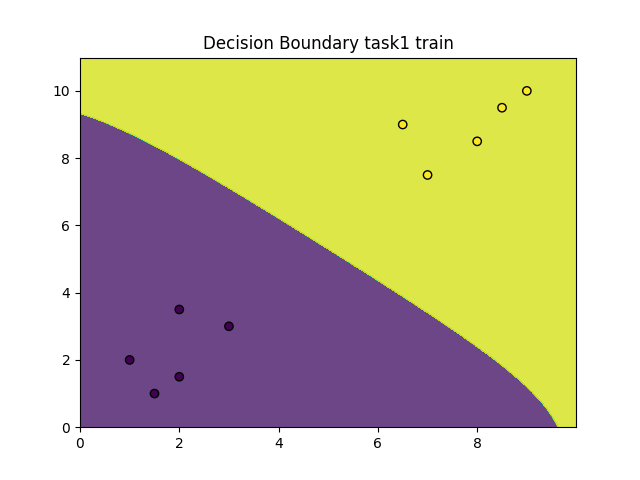
\includegraphics[width=\textwidth]{HW03/Prob2/out/task1/decision_boundary_train.png}
        \caption{分类边界线图}
        \label{fig:decision_boundary_train}
    \end{minipage}
    \hfill
    \begin{minipage}{0.45\textwidth}
        \centering
        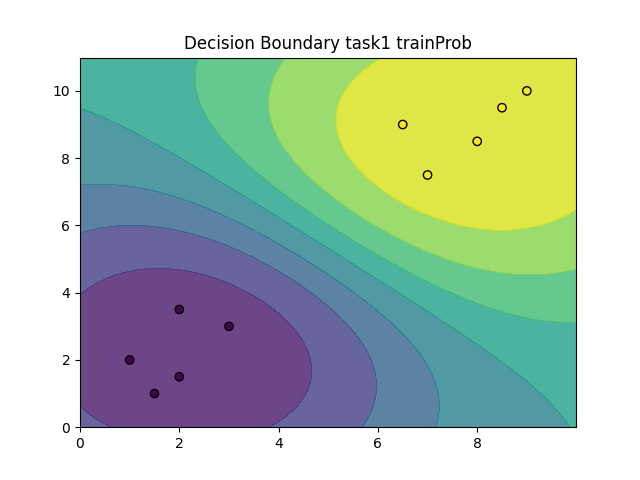
\includegraphics[width=\textwidth]{HW03/Prob2/out/task1/decision_boundary_trainProb.png}
        \caption{概率等高线图}
        \label{fig:decision_boundary_trainProb}
    \end{minipage}
    \hfill
\end{figure}
    
    \item \textbf{通过网格搜索优化提高模型的泛化能力} 

    我们通过网格搜索优化 SVM 的\textbf{惩罚参数} \(C\) 和\textbf{核系数} \( \gamma \) 。尝试 \( C \) 取值 \([0.1, 1, 10, 100]\) 和 \( \gamma \) 取值 \([0.1, 1, 10]\),找出最佳参数组合\( C = 0.1 \)和 \( \gamma  = 0.1\),输出了优化后训练准确率\(1.0000\)和支持向量索引\([0, 1, 2, 3, 4, 5, 6, 7, 8, 9]\)。
    
    \textbf{总结如下:}

    惩罚参数 \(C\)
    \begin{itemize} 
        \item \(C\) 是 SVM 中的正则化参数,控制着训练模型对误分类的惩罚力度。
        \item 较大的 \(C\) 值,对误分类的惩罚更大,模型会尽量减少训练错误;模型更复杂,可能会拟合训练数据中的噪声,导致过拟合,泛化能力下降。
        \item 较小的 \(C\) 值,对误分类的容忍度更高,允许部分训练错误;模型更简化,可能欠拟合,但泛化能力可能提高。
    \end{itemize}
    核系数 \(\gamma\)
    \begin{itemize} 
        \item \(\gamma\) 控制 RBF(径向基函数)核函数的影响范围,决定单个训练样本对决策边界的影响。
        \item 较大的 \(\gamma\) 值,单个样本的影响范围小,决策边界更灵活;模型复杂度增加,可能紧贴训练数据,容易过拟合。
        \item 较小的 \(\gamma\) 值,单个样本的影响范围大,决策边界更平滑;模型复杂度降低,可能欠拟合。
    \end{itemize}
    \textbf{综合来看:}较小的 \(C\) 和 \(\gamma\) 值导致模型简单,决策边界平滑,泛化能力较好。在训练集上准确率高,但存在过拟合的可能性,应结合验证集或测试集评价模型性能。适当的参数选择使模型不过于复杂,避免过拟合,从而在未知数据上保持良好的性能。
\end{enumerate}

\vspace{3em}

\section*{三. (20 分) 朴素贝叶斯分类器}
一家电商公司希望通过用户评论的关键词来预测评论的情感(\textbf{正面} 或 \textbf{负面})。假设已经收集了一小部分用户评论,并从中提取出以下五个关键词作为特征:\textbf{“good”}、\textbf{“bad”}、\textbf{“quality”}、\textbf{“price”} 和 \textbf{“recommend”}。每条评论可以被标记为“正面”或“负面”。

\begin{table}[h!]\small
    \centering
    \begin{tabular}{|c|c|c|c|c|c|}
        \hline
        评论情感 & good 出现次数 & bad 出现次数 & quality 出现次数 & price 出现次数 & recommend 出现次数 \\
        \hline
        正面评论 & 50 & 5 & 45 & 20 & 60 \\
        \hline
        负面评论 & 10 & 30 & 5 & 25 & 2 \\
        \hline
    \end{tabular}
\end{table}

假设正面评论和负面评论的先验概率分别为 \( P(\text{正面评论}) = 0.7 \) 和 \( P(\text{负面评论}) = 0.3 \)。

\subsection*{问题}

\begin{enumerate}
    \item \textbf{(8分)} 基于上述数据,使用\textbf{拉普拉斯修正}(\(\alpha = 1\))计算以下条件概率:
        \begin{itemize}
            \item \( P(\text{good} | \text{正面评论}) \)
            \item \( P(\text{bad} | \text{正面评论}) \)
            \item \( P(\text{quality} | \text{正面评论}) \)
            \item \( P(\text{price} | \text{正面评论}) \)
            \item \( P(\text{recommend} | \text{正面评论}) \)
        \end{itemize}
    同时,计算上述特征在负面评论下的条件概率。

    \item \textbf{(12分)} 假设我们有一条新评论 \( X = \{\text{good}, \text{quality}, \text{price}\} \),请使用朴素贝叶斯分类器计算该评论属于\textbf{正面评论}和\textbf{负面评论}的后验概率 \( P(\text{正面评论} | X) \) 和 \( P(\text{负面评论} | X) \),并根据计算结果确定该评论的情感类别。
\end{enumerate}

\textbf{提示}:
\begin{itemize}
    \item 本题的答案请以分式或者小数点后两位的形式给出,比如P=0.67.
    \item 在计算条件概率时,请注意考虑拉普拉斯修正后的分母变化。
    \item 最终的后验概率可以使用贝叶斯公式结合条件独立性假设:
    \[
    P(y|X) = \frac{P(y) \cdot P(X|y)}{P(X)}
    \]
    因为 \( P(X) \) 是相同的常数项,比较 \( P(y) \cdot P(X|y) \) 即可。
\end{itemize}

\textbf{\large 解:}


\vspace{3em}

\section*{四. (30 分) EM算法}
假设有一个包含 6 次硬币抛掷结果的数据集,记录了每次抛掷是否得到“正面”:
\[
X = \{\text{正面, 正面, 反面, 正面, 反面, 反面}\}
\]
假设这些结果是由两枚硬币 A 和 B 生成的,每次抛掷时选择使用硬币 A 或 B 的概率均为 \(0.5\)。然而,具体每次抛掷使用的是哪一枚硬币是未知的。硬币 A 和 B 的正面概率分别为 \( \theta_A \) 和 \( \theta_B \)。我们的目标是通过 EM 算法估计这两枚硬币的正面概率 \( \theta_A \) 和 \( \theta_B \)。

已知:
1. 初始参数:硬币 A 的正面概率 \( \theta_A^{(0)} = 0.6 \) 和硬币 B 的正面概率 \( \theta_B^{(0)} = 0.5 \)。
2. 每次抛掷使用硬币 A 和硬币 B 的概率均为 0.5,即 \( P(A) = 0.5 \) 和 \( P(B) = 0.5 \)。

请通过一轮 EM 算法的迭代步骤,估计硬币 A 和 B 的正面概率 \( \theta_A \) 和 \( \theta_B \)。本题的答案请以分式或者小数点后两位的形式给出,比如P=0.67.

\subsection*{问题:}

\begin{enumerate}
    \item \textbf{E步}(15分):对于每一次抛掷结果,使用当前的参数估计值(\( \theta_A^{(0)} \) 和 \( \theta_B^{(0)} \)),计算该结果由硬币 A 和硬币 B 生成的后验概率,即每次抛掷属于硬币 A 和硬币 B 的“软分配”概率。
    
    请计算以下内容:
    \begin{itemize}
        \item 在第 1 次到第 6 次抛掷中,每个结果(正面或反面)由硬币 A 生成的概率 \( P(A | x_i) \)。
        \item 每个结果由硬币 B 生成的概率 \( P(B | x_i) \)。
    \end{itemize}

    \item \textbf{M步}(15分):基于 E 步计算出的“软分配”概率,计算硬币 A 和 B 的正面和反面出现的期望次数,并更新硬币 A 和 B 的正面概率 \( \theta_A \) 和 \( \theta_B \)。

    请计算以下内容:
    \begin{itemize}
        \item 硬币 A 的正面和反面期望出现次数,并据此更新硬币 A 的正面概率 \( \theta_A^{(1)} \)。
        \item 硬币 B 的正面和反面期望出现次数,并据此更新硬币 B 的正面概率 \( \theta_B^{(1)} \)。
    \end{itemize}
\end{enumerate}

\textbf{\large 解:}


\end{document}
